\chapter{Разработка системы}

Прежде чем приступить к описанию процесса разработки, вернемся к рассмотрению выбранных технологий для реализации системы и обозначим решаемые с их помощью задачи.

В качестве архитектуры взаимодействия клиента и сервера выбран паттерн REST. Он позволяет использовать стандартные HTTP-методы для вызова методов API. Сервер разрабатывался на языке Python с помощью веб-фреймворка Django. Выбор обусловлен высоким уровнем модульности, благодаря чему возможно функциональное разделение сервера и, как следствие, независимая техническая поддержка частей, а также большой выбор билиотек, решающих рутинные задачи.

Клиентская часть, помимо HTML и CSS, содержит код JavaScript, необходимый для обеспечения интерактивности взаимодействия клиента с приложением. Здесь применен подход рендеринга со стороны клиента, что уменьшает нагрузку на веб-сервер. С помощью библиотеки React были построены основные элементы управления, Redux позволил реализовать паттерн «однонаправленный поток данных», что позволяет структурировать данные и обеспечить их актуальность для предоставления представлениям. Графическое построение конечных автоматов реализовано с использованием библиотеки D3, ориентированной на визуализацию данных через SVG.

\section{Сервер}

Сервер состоит из двух Django-приложений: 

\begin{itemize}
	\item \textit{model\_checker} -- приложение, реализующее выдачу статических файлов;
	\item \textit{api} - приложение, реализующее обработку запросов к API, включая запуск процесса NuSMV и выдачу результата выполнения.
\end{itemize}

Также в разработке использовались сторонние приложения: \textit{rest\_framework}, предоставляющий инструменты создания Web API в соответствии с принципами REST, и \textit{webpack\_loader}, необходимый для загрузки JavaScript bundle-файлов. Фрагмент конфигурационного файла приведен в листинге \ref{lst:config}.

\begin{lstlisting}[language=Python, 
label=lst:config, 
caption={Фрагмент конфигурационного файла Django.}]
INSTALLED_APPS = [
	'django.contrib.auth',
	'django.contrib.contenttypes',
	'django.contrib.staticfiles',
	'webpack_loader',
	'model_checker',
	'api',
	'rest_framework',
]
\end{lstlisting}

\subsection{Приложение \textit{api}}

Данное приложение, помимо генерируемых Django модулей, содержит две директории, необходимые для реализации обработки запросов к методам API:

\begin{itemize}
	\item \textit{~/bin/} -- содержит исполняемый файл модел-чекера NuSMV;
	\item \textit{~/sandbox/} -- содержит сгенерированные файлы исходного кода описания верифицируемой модели.
\end{itemize}

Обработка запроса происходит в модуле \textit{views.py}. Данную рекомендацию дают разработчики библиотеки Django REST Framework. В данном модуле реализовано 5 функций:

\begin{itemize}
	\item \textit{run\_simulation(request, flags)} -- запускает процесс NuSMV в интерактивном режиме и, в зависимости от флагов, передает в стандартный поток ввода процесса необходимые команды. По завершении возвращает информацию, предоставленную стандартным потоком вывода. Параметр \textit{request} представляет собой строку, содержащую переданный клиентом в теле запроса исходный код модели на языке SMV. Параметр \textit{flags} представляет собой флаги, используемые при запуске NuSMV.
	\item \textit{run\_verification(request)} -- запускает процесс NuSMV в обычном режиме, т.е. в режиме верификации модели. По завершении возвращает информацию, предоставленную стандартным потоком вывода. Параметр \textit{request} представляет собой строку, содержащую переданный клиентом в теле запроса исходный код модели на языке SMV. 
	\item \textit{create\_file(source\_code)} -- функция, создающая файл исходного кода SMV для последующей передачи процессу NuSMV. Параметр \textit{source\_code} -- строка, содержащая описание модели. Для генерации названия файла используется шаблон вида \textit{"smv<hash>.smv"}, где \textit{<hash>} -- хэш-сумма параметра \textit{source\_code}, вычисленная по алгоритму SHA-256. Возвращает путь к файлу в виде строки.
	\item \textit{create\_command(filename, flags)} -- возвращает массив строк, которые впоследствии будут переданы процессу NuSMV через именованный канал.
	\item \textit{run\_in\_command\_line(commands, nusmv\_commands)} -- функция, создающая новый процесс, в котором происходит запуск NuSMV. Параметр \textit{commands} является массивом строк, полученным с помощью функции \textit{create\_command(filename, flags)}. Параметр \textit{nusmv\_commands} -- массив комманд интерактивного режима NuSMV.
\end{itemize}

К функциям \textit{run\_simulation} и \textit{run\_verification} подключены декораторы \textit{@api\_view} с параметром \textit{'POST'}. Данный декоратор является частью библиотеки Django REST Framework и необходим при вызове обработчиков запросов. Для разделения методов симуляции и верификации модели используется механизм роутинга, который предполагает использование разных URL для вызываемых методов. Привязка обработчиков к URL происходит в модуле urls.py, фрагмент которого приведен в листинге \ref{lst:url_assign}.

\begin{lstlisting}[language=Python, 
label=lst:url_assign, 
caption={Фрагмент файла urls.py.}]
urlpatterns = [
	url(r'^simulate/$', run_simulation, name='run_simulation'),
	url(r'^verify/$', run_verification, name='run_verification')
]
\end{lstlisting}

Как упоминалось выше, создание процесса NuSMV и взаимодействие с ним происходит в методе \textit{run\_in\_command\_line}. В нем используется класс \textit{Popen} пакета \textit{subprocess}. Данный класс предоставляет возможность создания процесса и привязки к его стандартным потокам ввода/вывода именованного канала, благодаря которому мы получаем информацию о выполнении NuSMV в процессе сервера.

\subsection{Приложение \textit{model\_checking}}

Данное приложение отвечает за выдачу статических файлов клиенту. В корневой директории приложения, помимо сгенерированных фреймворком, содержатся две папки:

\begin{itemize}
	\item \textit{~/static/}, содержащая статические файлы JavaScript и CSS, которые будут рассмотрены подробнее в разделе \ref{sec:client};
	\item \textit{~/templates/}, содержащая файлы шаблонов.
\end{itemize} 

Фреймворк Django дополняет синтаксис HTML, что позволяет строить шаблоны страниц, в которых загрузка динамических данных происходит с помощью специального синтаксиса -- DTL (Django Template Language). Разрабатываемое приложение содержит всего одну страницу, шаблон которой приведен в листинге \ref{lst:template}. Особо выделим строки, содержащие синтаксис DTL, и опишем выполняемые ими функции:

\begin{itemize}
	\item [(1)]: Инициализация приложения, необходимого для загрузки JavaScript файла, сгенерированного системой сборки Webpack (подробнее в разделе \ref{sec:client}).
	\item [(2)]: Инициализация инструментов загрузки статических файлов.
	\item [(7)]: Загрузка статического файла CSS.
	\item [(20)]: Загрузка статического файла JavaScript.
\end{itemize}

\begin{lstlisting}[language=HTML, 
label=lst:template, 
caption={Файл main.html -- шаблон страницы.}]


<!DOCTYPE html>
<html lang="en">
	<head>
		<meta charset="UTF-8">
		<link rel="stylesheet" href="">
		<title> WebSMV </title>
	</head>
	<body>
		<section>
			<div class="app-container">
				<div id="dropdown-container"></div>
				<div id="state-editor-container"></div>
				<div id="workspace-container"></div>
				<div id="run-config-container"></div>
				<div id="source-code-editor-container"></div>
				<div id="results-container"></div>
			</div>
			
		</section>
	</body>
</html>
\end{lstlisting}

\section{Клиент}\label{sec:client}

Разработчики React придерживаются разделения компонентов на два типа: \textit{\textbf{«глупые»} компоненты} -- сущности, занимающиеся исключительно рендером элементов HTML и вызывающие обработку событий с помощью механизма обратных вызовов, \textit{\textbf{«умные»} компоненты} -- инкапсулируют в себе «глупые» компоненты и передают им ссылки на функции и данные.

Здесь и далее примем \textit{«умные»} \textit{компоненты} как \textit{контейнеры}, а \textit{«глупые»} как \textit{компоненты}.

\subsection{Компоненты}

\textbf{StateEditor} -- реализует работу с множеством состояний конечного автомата. Активируется при выборе конкретного состояния. Состоит из поля ввода названия переменной, раскрывающегося списка типов переменных и кнопки добавления.Стоит отметить, что состав компонента StateEditor изменяется при изменении типа переменной. Так, для переменной типа массив компонент отображает также диапазон используемых индексов и раскрывающийся список возможных типов элементов массива, а для типа перечисление отображается поле ввода нового элемента перечисления, кнопка его добавления и список возможных значений, поддерживающий возможность удаления.


\begin{figure}[ht]
	\centering
	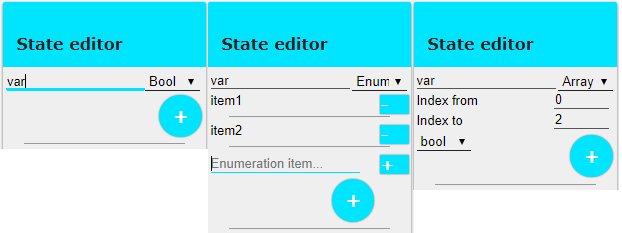
\includegraphics[width=0.8\textwidth]{fig/state_editor.png}
	\caption{Вид компонента StateEditor для трех типов переменных.}
	\label{fig:state_editor}
\end{figure}

\textbf{StateItems} -- реализует отображение и редактирование списка атомарных высказываний, соответствующих выбранному состоянию. Состоит из списка атомарных высказываний, каждый элемент которой имеет текстовое поле, отображающее название переменной и ее тип, раскрывающийся список возможных значений переменной и кнопку удаления переменной из множества состояний. Для переменной типа массив компонент отображает множество выпадающих списков, содержащих допустимые для элементов массива значения.


\begin{figure}[htbp]
	\centering
	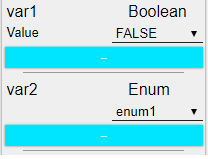
\includegraphics[width=0.4\textwidth]{fig/state_item.png}
	\caption{Вид компонента StateItem.}
	\label{fig:state_item}
\end{figure}

\textbf{TransitionView} -- отображает отношение перехода, т.е. имена измененных после перехода переменных и их новые значения. Состоит из списка текстовых полей.

\textbf{SimFlagsBox} -- реализует возможность настройки флагов, используемых при симуляции.

\textbf{CtlBox/LtlBox} -- компоненты, реализующие создание и отображение спецификаций. В зависимости от выбранного типа темпоральной логики изменяются доступные кнопки.

\begin{figure}[htbp]
	\centering
	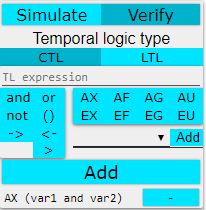
\includegraphics[width=0.4\textwidth]{fig/tl_box.png}
	\caption{Вид компонента CtlBox.}
	\label{fig:tl_box}
\end{figure}

\subsection{Контейнеры}

В каждом из контейнеров реализовано две функции Redux: 

\begin{itemize}
	\item \textit{mapStateToProps} -- устанавливает соответствие между объектами-свойствами контейнера и объектами хранилища;
	\item \textit{mapDispatchToProps} -- устанавливает соответствие между объектами-функциями контейнера и функциями создателями действий.
\end{itemize}

Таким образом происходит присоединение представления к схеме однонаправленного потока данных. Рассмотрим подробнее разработанные контейнеры.

\textbf{StateEditorContainer} -- контейнер, инкапсулирующий компоненты отображения и редактирования состояний и переходов. При выборе состояния отображает \textit{StateEditor} и \textit{StateItem}, при выборе перехода отображает \textit{EdgeView}. Использует следующие редьюсеры:

\begin{itemize}
	\item WorkspaceReducer,
	\item StateItemReducer,
	\item StateEditorReducer.
\end{itemize}

\textbf{WorkspaceContainer} -- контейнер, инкапсулирующий в себе главный SVG элемент блока построения конечных автоматов. Содержит объект D3Graph (подробнее в разделе \ref{sec:d3}). Работает с WorkSpaceReducer.

\textbf{TlContainer} -- контейнер, отображающий CtlBoc или LtlBox в зависимости от полученного свойства.

\textbf{RunConfigContainer} -- контейнер, содержащий в себе кнопки переключения режима (симуляция/верификация). В режиме верификации отображает кнопки переключения типа темпоральной логики и \textit{TlContainer}.

\textbf{SourceCodeContainer} -- текстовое поле, отображающее сгенерированный исходный код на языке SMV.

\textbf{ExecutionResultContainer} -- текстовое поле, содержащее вывод программы NuSMV, полученный из тела ответа сервера.

\subsection{Модель редьюсеров}

В приложении используется 6 редьюсеров.

\textbf{StateItemReducer} -- редьюсер, необходимый для создания новой переменной состояния. Описание полей объекта приведено в таблице \ref{tab:state_item}.

\begin{lstlisting}[language=Java,
caption={Инициализация состояния StateItemReducer.}]
const initialState = {
	stateItem:{
		stateName: '',
		type: 'bool',
		value: '',
		range: [],
		arrayType: ''
	}
};
\end{lstlisting}

\begin{table}[ht]
	\caption{Описание полей StateItemReducer.}\label{tab:state_item}
	\centering
	\begin{tabular}{|m{2.5 cm}|m{1.5 cm}|m{4.75 cm}|}
		\hline
		Название & Тип & Описание \\
		\hline
		stateName & Строка & Название переменной \\
		\hline
		type & Строка & Тип переменной \\
		\hline
		value & Строка / массив & Значение переменной; массив значений для типа array \\
		\hline
		range & Массив & Диапазон возможных значений; нижний и верхний индексы для типа array \\
		\hline
		arrayType & Строка & Тип элементов массива; пустая строка, если $type\neq'array'$\\
		\hline
	\end{tabular}
\end{table}

\newpage

\textbf{StateEditorReducer} -- работает с массивом переменных состояния, каждый элемент которого является объектом StateItem.

\begin{lstlisting}[language=Java,
caption={Инициализация состояния StateEditorReducer.}]
const initialState = {
	states:[]
};
\end{lstlisting}

\textbf{WorkspaceReducer} -- основной редьюсер, работающий моделью конечного автомата, представленной в виде графа, генерируемым исходным кодом описания, а также генераторами названий состояний и переходов. Подробнее поля объекта состояния рассмотрены в таблице \ref{tab:workspace}.

\begin{lstlisting}[language=Java,
caption={Инициализация состояния WorkspaceReducer.}]
const initialState = {
	graph: {
		vertices:[],
		edges: [],
		initVertex: {},
		selected: ''},
	enums: [],
	vertexGenerator: 0,
	edgeGenerator: 0,
	sourceCode: '',
};
\end{lstlisting}

\begin{table}[ht]
	\caption{Описание полей WorkspaceReducer.}\label{tab:workspace}
	\centering
	\begin{tabular}{|m{2.5 cm}|m{1.5 cm}|m{4.75 cm}|}
		\hline
		Название & Тип & Описание \\
		\hline
		graph & Объект & Объектное представление модели конечного автомата \\
		\hline
		vertices & Массив & Массив объектов вершин графа \\
		\hline
		edges & Массив & Массив объектов ребер графа \\
		\hline
		initVertex & Объект & Инициализирующее состояние конечного автомата \\
		\hline
		selected & Строка & Название текущей выбранной вершины или ребра \\
		\hline
		enums & Массив & Массив объектов переменных, типом которых является \textit{enumeration} \\
		\hline
		vertexGenerator & Целое число & Генератор номеров вершин \\
		\hline
		edgeGenerator & Целое число & Генератор номеров ребер \\
		\hline
		sourceCode & Строка & Исходный код описания модели на языке SMV \\
		\hline
	\end{tabular}
\end{table}

\textbf{TlReducer} -- работает с типом выбранной пользователем темпоральной логики.

\begin{lstlisting}[language=Java,
caption={Инициализация состояния TlReducer.}]
const initialState = {
	tlType:'ctl'
};
\end{lstlisting}

\textbf{TlBoxReducer} -- работает с вводимой пользователем в CtlBox/LtlBox формулой.

\newpage

\begin{lstlisting}[language=Java,
caption={Инициализация состояния TlBoxReducer.}]
const initialState = {
	formula: ' '
};
\end{lstlisting}

\textbf{RunConfigReducer} -- редьюсер, используемый в контейнере \textit{RunConfigContainer}. Описание полей приведено в таблице \ref{tab:run_config}.

\begin{lstlisting}[language=Java,
caption={Инициализация состояния RunConfigReducer.}]
const initialState = {
	runMode: 'sim',
	simFlags: {},
	ctlFormulas: [],
	ltlFormulas: [],
	result: ''
};
\end{lstlisting}

\begin{table}[ht]
	\caption{Описание полей RunConfigReducer.}\label{tab:run_config}
	\centering
	\begin{tabular}{|m{2.5 cm}|m{1.5 cm}|m{5 cm}|}
		\hline
		runMode & Строка & Тип операции NuSMV: симуляция или верификация \\
		\hline
		simFlags & Объект & Объект, содержащий флаги NuSMV и их значения \\
		\hline
		ctlFormulas & Массив & Массив введенных пользователем CTL-формул, представленных в виде строк\\
		\hline
		ltlFormulas & Массив & Массив введенных пользователем LTL-формул, представленных в виде строк\\
		\hline
		result & Строка & Полученный от сервера вывод программы NuSMV\\
		\hline
	\end{tabular}
\end{table}

\subsection{Создатели дейтсвий}

Создатели действий (Action Creators) -- чистые функции, принимающие измененную часть хранилища состояния и возвращающие новый объект, содержащий тип действия и полученный параметр. В таблице \ref{tab:actions} описаны основные типы используемых действий.

\begin{table}[ht]
	\caption{Основные типы действий.}\label{tab:actions}
	\centering
	\begin{tabular}{|m{4.5 cm}|m{5.5 cm}|}
		\hline
		Тип действия & Описание \\
		\hline
		CHANGE\_FORMULA & Изменение формулы в редакторе спецификаций \\
		\hline
		ADD\_LTL& Добавление LTL формулы к списку спецификаций  \\
		\hline
		ADD\_VERTEX& Добавление новой вершины к графу \\
		\hline
		MOVE\_VERTEX& Перенос вершины в поле построения \\
		\hline
		ADD\_EDGE& Добавление нового ребра к графу \\
		\hline
		SET\_INIT& Установка инициализирующей вершины графа \\
		\hline
		CHANGE\_SELECTED& Изменение выбранного пользователем элемента графа \\
		\hline
		ADD\_STATE\_TO\_GRAPH& Добавление новой переменной состояния в граф \\
		\hline
	\end{tabular}
\end{table}

\subsection{Поле построения конечных автоматов} \label{sec:d3_impl}

Для отрисовки поля построения конечных автоматов и взаимодействия с ним используется библиотека D3. Реализован класс D3graph, список методов и их описание приведены в таблице \ref{tab:d3}.

\begin{table}[ht]
	\caption{Описание методов класса D3graph.}\label{tab:d3}
	\centering
	\begin{tabular}{|m{4 cm}|m{6 cm}|}
		\hline
		\textbf{Сигнатура метода} & \textbf{Описание} \\
		\hline
		
		\textit{constructor(props)} & Конструктор класса. Параметр \textit{props} -- объект, содержащий представление конечного автомата, а также ссылки на создателей дейтсвий.\\
		
		\hline
		
		\textit{update(props)} & Отвечает за обновление визуализации конечного автомата в соответствии с входными данными. Параметр \textit{props} -- объект того же вида, что и в конструкторе класса. Данный метод вызывается каждый раз при обновлении Redux-хранилища.\\
		
		\hline
		
		\textit{createMarkup()} & Создает разметку поля построения. Вызывается один раз при инициализации инкапсулирующего поле контейнера  \textit{WorkspaceContainer}. \\
		
		\hline
		
		\textit{on<Elem>Click()} & Обработчики клика на элемент SVG, где \textit{<Elem>} -- целевой элемент SVG клика, может принимать три значения: \textit{Root} -- корневой SVG элемент, \textit{Vertex} -- группа элементов, представляющих вершину графа, \textit{Edge} -- группа элементов, представляющих ребро графа.\\
		
		\hline
		
		\textit{on<Elem>ContextClick()} & Обработчики контекстного клика на элемент SVG, где \textit{<Elem>} соответствует описанному в группе методов \textit{on<Elem>Click()}.\\
		
		\hline
		
		\textit{onDrag()/onDrop()} & Обработчики событий перемещения элемента вершины графа. \\
		
		\hline
		
		\textit{on<Action>Click()} & Обработчики клика на элемент контексного меню. \\
		
		\hline
	\end{tabular}
\end{table}

\begin{figure}[htbp]
	\centering
	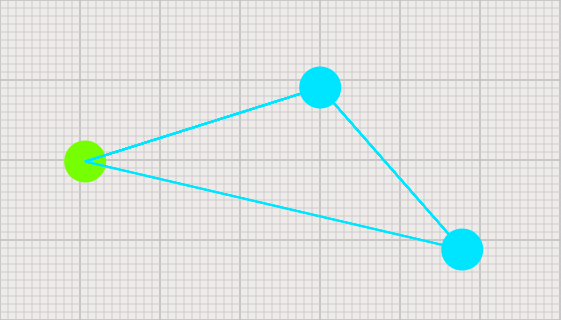
\includegraphics[width=0.8\textwidth]{fig/graph.png}
	\caption{Вид поля построения конечных автоматов.}
	\label{fig:graph}
\end{figure}

Построение происходит путем добавления SVG элементов средствами библиотеки D3. Основой для представления вершины графа служит SVG circle, для представления ребра -- SVG line. Как было сказано в разделе \ref{sec:d3}, библиотека ориентирована на визуализацию данных, которые связываются с элементами с помощью метода \textit{data(array)}, где \textit{array} является массивом данных. Последующая обработка происходит в определяемых пользователем библиотеки функциях посредством передачи ссылок на обработчики данных или лямбда-выражений. В листинге \ref{lst:line_creation} приведен фрагмент кода, реализующего добавление линий разметки поля построения.

\begin{lstlisting}[language=Java,
				   label=lst:line_creation,
				   caption={Добавление разметки поля построения конечных автоматов.}]
let lines = root.append('g').selectAll('line')
	// steps -- массив координат отступов между линиями разметки 
	// по оси ординат
	.data(steps) 
	.enter()
	.append('line')
	.attr('class', 'markdown')
	.attr('x1', (d)=>{return d;})
	.attr('x2', (d)=>{return d;})
	.attr('y1', 0)
	// height -- высота поля построения
	.attr('y2', height);
\end{lstlisting}

\subsection{Взаимодействие React и D3}

Совместное использование библиотек React и D3 осложнено реализацией совместного использования и изменения объектного представления конечного автомата. Компонент React реализован придерживаясь концепции элементов с жизненным циклом, в то время как D3 выполняет непосредственную вставку элементов в корневой элемент SVG. Для актуализации отображаемой информации был реализован метод \textit{D3graph.update(props)}. Данный метод, как описано в \ref{sec:d3_impl}, производит переотрисовку всех элементов конечного автомата в соответствии с принятым как параметр объектом. Данный метод вызывается в одном из методов жизненного цикла React-компонента -- \textit{React.Component.componentDidUpdate()}.

% картинка

\subsection{Сборка фронэнд-части проекта}

Прежде чем приступить к сборке проекта, рассмотрим структуру проекта в файловой системе (рисунок \ref{lst:dir_tree}). 

\begin{lstlisting}[language=Java,
label=lst:dir_tree,
caption={Дерево директорий проекта.}]
|---bundles
|	|---main<hashcode>.js
|
|---css
|	|---main.css
|
|---js
    |---actions
    |---components
    |---containers
    |---d3
    |---reducers
    |---store
    |---util
    |---app.js
\end{lstlisting}

Рассмотрим подробнее приведенные выше директории:

\begin{itemize}
	\item \textit{bundles} содержит главный JavaScript файл, генерируемый системой сборки. Данный файл передается сервером клиенту.
	\item \textit{css} содержит CSS файл, в котором описаны все используемые классы элементов.
	\item \textit{js} содержит JavaScript файлы исходного кода для разработчиков.
	\item \textit{actions} содержит функции, реализующие создание действий Redux.
	\item \textit{components} -- содержит классы React компонентов.
	\item \textit{containers} -- содержит классы React контейнеров.
	\item \textit{d3} -- содержит класс D3graph, реализующий отрисовку поля построения конечного автомата средствами библиотеки D3.
	\item \textit{reducers} -- содержит описания редьюсеров Redux.
	\item \textit{store} -- содержит конфигурационный файл хранилища Redux.
	\item \textit{util} -- содержит вспомогательные файлы, например, ArrayAdditions.js, в котором реализован поиск элемента в массиве объектов по одному из полей.
\end{itemize}

Данная структура проекта предоставляет большую наглядность, что упрощает разработку проекта. Однако такое разбиение проекта на модули усложняет процесс подключения скриптов в HTML файле. Также, вследствие отсутствия поддержки браузерами, использование стандарта ECMA Script 6 требует трансляцию кода в соответствии со стандартом EMCA Script 5. Использование различных библиотек влечет за собой большое количество внешних зависимостей, подключение которых вручную -- достаточно трудоемкая задача. Для решения данных проблем используется система сборки Webpack. Данная система позволяет транслировать код, написанный с помощью разных стандартов как JavaScript, так и CSS, в код, соответствующий поддерживаемым большинством браузером стандартам. Webpack использует механизм загрузчиков: с помощью их конфигурации (листинг \ref{lst:webpack}) система автоматически выполняет необходимые операции по трансляции. 

\begin{lstlisting}[language=Java,
label=lst:webpack,
caption={Фрагмент конфигурационного файла Webpack.}]
loaders: [
	//a regexp that tells webpack use the following loaders on all 
	//.js and .jsx files
	{
		test: /\.jsx?$/,
		loader: 'babel-loader', 
		query: {
			//specify that we will be dealing with React code
			presets: ['react', 'es2015', 'stage-0'],
			env: {
				development: {
					presets: ["react-hmre"]
				}
			}
		}
	}
],
\end{lstlisting}





